\subsubsection{\roofunit}
    %
    The {\roofunit} gadgets consist of two parts, the scaffolding and the shingles.
    %
    The scaffolding is responsible for assembling a path from the top of the final last digit and adding a height of 15 tiles to the current (final) counter row.
    %
    Since the most significant digit is positioned at a different height within a digit region depending on how many digits
    are in the MSR, the {\roofscaffolding} gadget's height must account for this.
    %
    If the MSR has 3 digits, the height is only 15 tiles.
    %
    If the MSR has 2 digits, the height is $30 + 12l + 15$ tiles.
    %
    Otherwise, if the MSR has 1 digit the height is $2 (30 + 12l) + 15$ tiles.
    %



    \begin{itemize}
        \item If case 1: create
        $\begin{aligned}[t]
            \roofscaffolding(& \left\langle {\tt RoofScaffolding}, 1, {\tt halt}, {\tt msr}, {\tt msd} \right\rangle,
                               \left\langle {\tt RoofShingle},     0                                   \right\rangle \;)
        \end{aligned}$\\from the gadget shown in Figure~\ref{fig:roof_unit_1}.

        \item If case 2: create
        $\begin{aligned}[t]
            \roofscaffolding(& \left\langle {\tt RoofScaffolding}, 2, {\tt halt}, {\tt msr}, {\tt msd} \right\rangle,
                               \left\langle {\tt RoofShingle},     0                                   \right\rangle \;)
            \end{aligned}$\\from the gadget shown in Figure~\ref{fig:roof_unit_2}.

        \item If case 3: create
        $\begin{aligned}[t]
            \roofscaffolding(& \left\langle {\tt RoofScaffolding}, 3, {\tt halt}, {\tt msr}, {\tt msd} \right\rangle,
                               \left\langle {\tt RoofShingle},     0                                   \right\rangle \;)
            \end{aligned}$\\from the gadget shown in Figure~\ref{fig:roof_unit_3}.

        \item For each $i = 0,\ldots,\ceil*{\frac{d}{3}} - 1$, create
        $\begin{aligned}[t]
            \roofshingle(& \left\langle {\tt RoofShingle}, i     \right\rangle,
                           \left\langle {\tt RoofShingle}, i + 1 \right\rangle \;)
            \end{aligned}$\\from the gadget shown in Figure~\ref{fig:roof_unit_right_shingles}.

        \item If $k$ is odd, we add one additional tile to the rightmost shingle, with a west glue
              labeled\\ $\left\langle {\tt RoofShingle}, \ceil*{\frac{d}{3}} \right\rangle$.
    \end{itemize}



\begin{figure}[H]
    \centering
    \subcaptionbox{
        Case 1 - roof unit scaffolding.
        \label{fig:roof_unit_1}
    }{\makebox[0.24\textwidth][c]{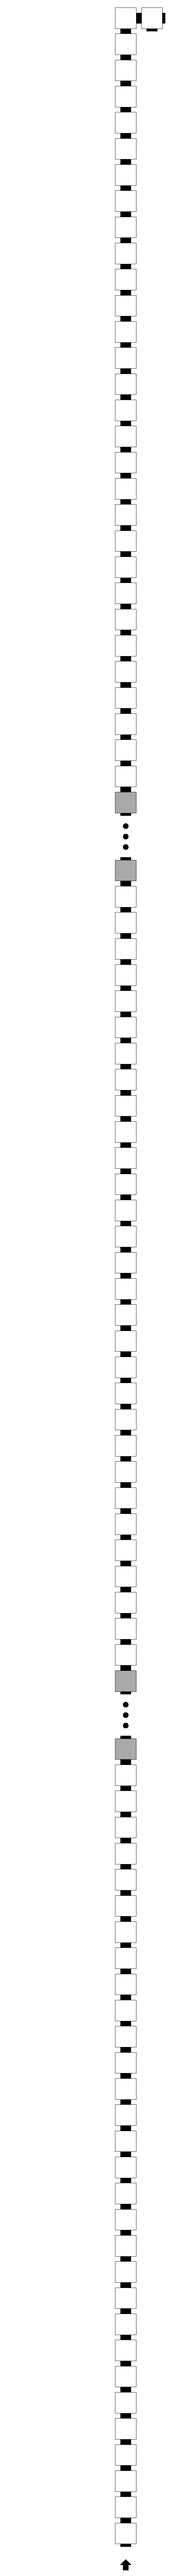
\includegraphics[width=0.45in]{roof_unit_1}}}%
    ~
    \subcaptionbox{
        Case 2 - roof unit scaffolding.
        \label{fig:roof_unit_2}
    }{\makebox[0.24\textwidth][c]{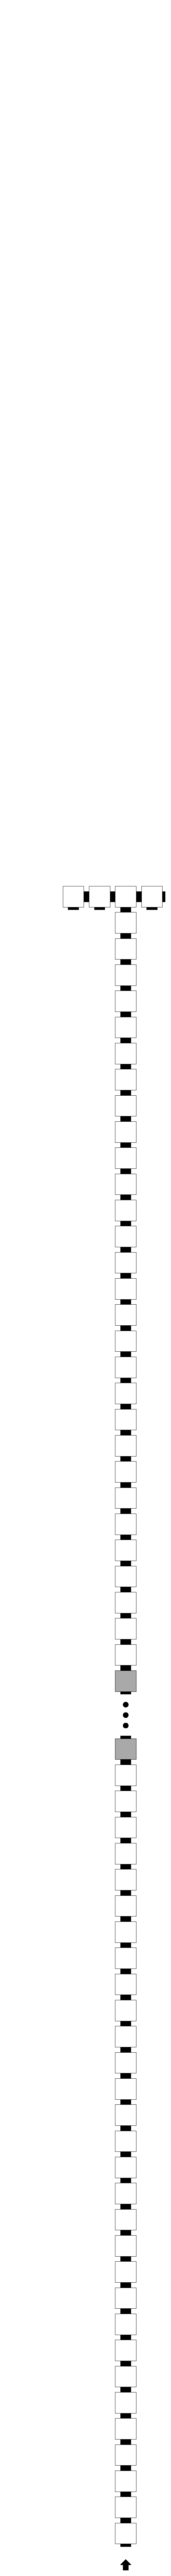
\includegraphics[width=0.45in]{roof_unit_2}}}%
    ~
    \subcaptionbox{
        Case 3 - roof unit scaffolding.
        \label{fig:roof_unit_3}
    }{\makebox[0.24\textwidth][c]{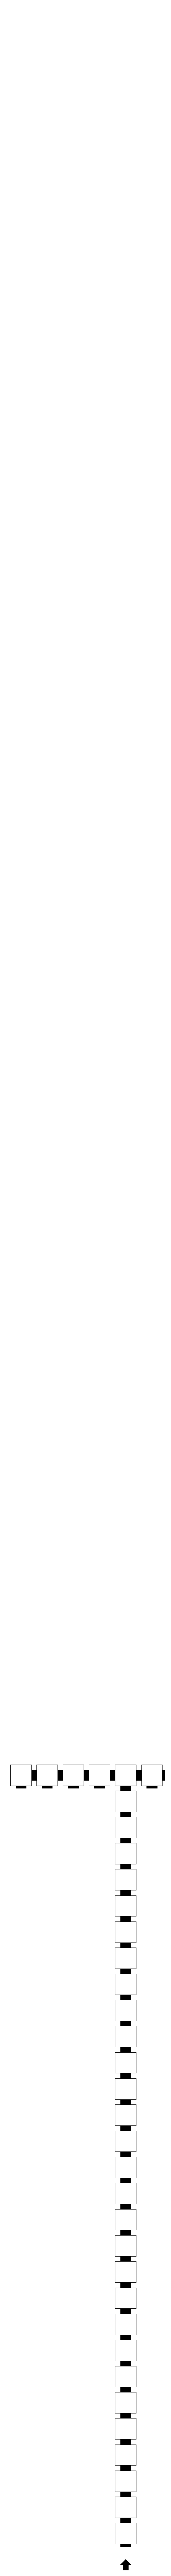
\includegraphics[width=0.45in]{roof_unit_3}}}%
    ~
    \subcaptionbox{
        Right shingles.
        \label{fig:roof_unit_right_shingles}
    }{\makebox[0.24\textwidth][c]{
\includegraphics[width=0.45in]{roof_unit_right_shingle}}}%
    ~
    \caption{\label{fig:roof_units} The {\roofunit} gadgets.}
\end{figure}